\subsection{Clearing the Air: Discover Noise Blanker Magic!}

\begin{tcolorbox}[colback=gray!10, colframe=black, title=E4E03`]
Which of the following types of noise are removed by a noise blanker? 
\begin{enumerate}[label=\Alph*.]
    \item Broadband white noise
    \item \textbf{Impulse noise}
    \item Hum and buzz
    \item All these choices are correct
\end{enumerate} \end{tcolorbox}

\subsubsection{Related Concepts}

A noise blanker is a specialized circuit used in radio communications to reduce or eliminate certain types of interference, primarily impulse noise. 

\subsubsection{Types of Noise}
Impulse noise is characterized by short bursts of energy over a wide bandwidth, such as electrical surges from nearby equipment or lightning. It can cause distortion in the received signal and degrade the quality of communication.

In contrast, broadband white noise is a type of noise that spans a wide frequency range and is generally continuous. This type of noise is not effectively removed by noise blankers. Hum and buzz are typically caused by AC line interference and while they can be irritating, they are not the primary focus for noise blankers.

\subsubsection{Important Concepts for Understanding Noise Blankers}
To effectively use and understand noise blankers, one should be familiar with:
\begin{itemize}
    \item The definitions of various types of electrical noise.
    \item The principles of signal processing and noise reduction techniques.
    \item Basic radio communication concepts, including modulation and demodulation.
\end{itemize}

In conclusion, the correct answer to the question regarding the type of noise removed by a noise blanker is impulse noise. The other types of noise, while they may interfere with radio communications, are not the primary concern of a noise blanker.

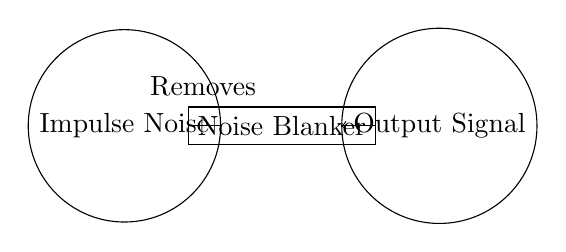
\begin{tikzpicture}
    \node[draw, circle] (noise) at (0,0) {Impulse Noise};
    \node[draw, rectangle] (blanker) at (2,0) {Noise Blanker};
    \node[draw, circle] (output) at (4,0) {Output Signal};
    
    \draw[->] (noise) -- (blanker) -- (output);
    \node at (1,0.5) {Removes};
\end{tikzpicture}
